\documentclass[11pt,a4paper,fleqn]{scrartcl}

\usepackage[utf8]{inputenc}
\usepackage[T1]{fontenc}
\usepackage[colorlinks=true, citecolor=blue, linkcolor=blue, filecolor=blue,urlcolor=blue]{hyperref}
\hypersetup{
     colorlinks   = true,
     citecolor    = gray
}
\usepackage{wrapfig}

\usepackage{caption}
\captionsetup{format=plain, indent=5pt, font=footnotesize, labelfont=bf}

\setkomafont{disposition}{\scshape\bfseries}

\usepackage{amsmath}
\usepackage{amssymb}
\usepackage{amsfonts}
\usepackage{bbm}
\usepackage{mathtools}
% \usepackage{epsfig}
% \usepackage{grffile}
%\usepackage{times}
\usepackage{palatino}
\usepackage{mathpazo}
\setlength\parindent{0pt}

%\usepackage{babel}
\usepackage{tikz}
\usepackage{paralist}
\usepackage{color}
\usepackage[top=3cm, bottom=2.5cm, left=2.5cm, right=3cm]{geometry}
%\setlength{\mathindent}{1ex}

% PGF
\usepackage{pgfplots}
\pgfplotsset{
  compat=newest,
  every axis/.append style={small, minor tick num=3}
}

%\usepackage[backend=biber,style=alphabetic,url=false,doi=false]{biblatex}
%\addbibresource{sheet01_biber.bib}
% \addbibresource{/home/coroa/papers/refs.bib}

\newcommand{\id}{\mathbbm{1}}
\newcommand{\NN}{{\mathbbm{N}}}
\newcommand{\ZZ}{{\mathbbm{Z}}}
\newcommand{\RR}{{\mathbbm{R}}}
\newcommand{\CC}{{\mathbbm{C}}}
\renewcommand{\vec}[1]{{\boldsymbol{#1}}}

\renewcommand{\i}{\mathrm{i}}

\newcommand{\expect}[1]{\langle\,#1\,\rangle}
\newcommand{\e}[1]{\ensuremath{\,\mathrm{#1}}}

\renewcommand{\O}{\mc{O}}
\newcommand{\veps}{\varepsilon}
\newcommand{\ud}[1]{\textup{d}#1\,}

\newcommand{\unclear}[1]{\color{green}#1}
\newcommand{\problem}[1]{\color{red}#1}

%=====================================================================
%=====================================================================
\begin{document}

\begin{flushright}
 \textbf{Energy System Modelling }\\
 {\small Karlsruhe Institute of Technology}\\
 {\small Institute for Automation and Applied Informatics}\\
 {\small Summer Term 2020}\\
\end{flushright}

 
 \vspace{-0.5em}
 \hrulefill
 \vspace{0.3em}

\begin{center}
 \textbf{\textsc{\Large Tutorial I: Time Series Analysis}}\\
 \small Will be worked on in the exercise session on Thursday, 4 June 2020.\\[1.5em]
\end{center}

\vspace{-0.8em}
\hrulefill
\vspace{0.8em}

%=============== ======================================================
\paragraph{Problem I.1 (programming) -- Data Analysis}~\\
%=====================================================================

The following data are made available to you on the course home
page\footnote{\url{https://nworbmot.org/courses/esm-2020/}} and the github repository \footnote{\url{https://github.com/lisazeyen/ESM_tutorial/tree/master/tutorial/01-tutorial-04.06.2020/notebooks/data}} :
\begin{verbatim}
  de_data.csv, gb_data.csv, eu_data.csv, (wind.csv, solar.csv, load.csv).
\end{verbatim}
They describe (quasi-real) time series for wind power generation \(W(t)\), solar power generation \(S(t)\) and load \(L(t)\) in Great Britain (GB), Germany (DE) and Europe (EU). The time step is \(1\e{h}\) and the time series are several years long.

\begin{enumerate}[(a)]
 \item Check that the wind and solar time series are normalized to 'per-unit of installed \mbox{capacity}', and that the load time series is normalized to MW.
 \item For all three regions, calculate the maximum, mean, and variance of the time series.
 \item For all three regions, plot the time series \(W(t)\),
       \(S(t)\),
       \(L(t)\) for a winter month (January) and a summer month (July).
 \item Resample the time series to daily, weekly and monthly data points and visualise them in plots. Can you identify some recurring patterns? 
 \item For all three regions, plot the duration curve for \(W(t)\), \(S(t)\), \(L(t)\).
 \item For all three regions, plot the probability density function of \(W(t)\), \(S(t)\), \(L(t)\).
 \item Recurring patterns of time series can also be visualised more rigorously by applying a Fourier Transform. Apply a (Fast) Fourier Transform to the the three time series $X \in W(t), S(t), L(t)$:
       \begin{equation*}
        \tilde{X}(\omega) = \int_0^T X(t) e^{\i \omega t} \,\ud t \, .
       \end{equation*}
       For all three regions, plot the energy spectrum
       $\left| \tilde{X}(\omega) \right|^2$ as a function of
       $\omega$. Discuss the relationship of these results with the
       findings obtained in (b)-(f).
 \item Normalize the time series to one, so that \(\expect{W} = \expect{S} = \expect{L} = 1\).
       Now, for all three regions, plot the mismatch time series
       \begin{equation*}
        \Delta(t) = \gamma \alpha W(t) + \gamma (1 - \alpha) S(t) - L(t)
       \end{equation*}
       for the same winter and summer months as in (c). Choose
       \(\alpha \in \{0.0, 0.5, 0.75, 1.0\}\) with \(\gamma = 1\),
       and $\gamma \in \{0.5, 0.75, 1.0, 1.25, 1.5\} $ with $\alpha = 0.75$.
       
       Which configuration entails the lowest mismatch on average and in extremes?       
       
 \item For all three regions, repeat (b)-(g) for the mismatch time series.
\end{enumerate}

\pagebreak
%=====================================================================
\paragraph{Problem I.2 (analytical) -- Effect of Seasonality}~\\
%=====================================================================

\begin{wrapfigure}[11]{r}{0pt}
 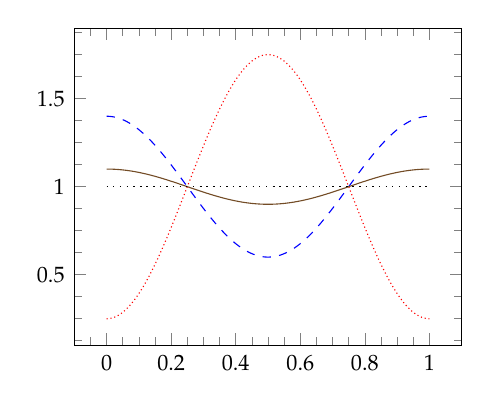
\begin{tikzpicture}
  \begin{axis}[
    domain=0:1, no markers, samples=200
    % xlabel = $x$, ylabel = $f(x)$
   ]
   \addplot+[dashed] {1 + 0.4 * cos(deg(2*pi*x))}; \label{figref:w}
   \addplot+[densely dotted] {1 - 0.75 * cos(deg(2*pi*x))}; \label{figref:s}
   \addplot+[solid] {1 + 0.1 * cos(deg(2*pi*x))}; \label{figref:l}
   \addplot+[dotted] {1}; \label{figref:1}
  \end{axis}
 \end{tikzpicture}
 \caption{Seasonal variations of wind and solar power generation
  \(W(t)\)
  \autoref{figref:w} and \(S(t)\)
  \autoref{figref:s}, and load \(L(t)\)
  \autoref{figref:l} around the mean \(1\) \ref{figref:1}.}
 \label{fig:seasonalvariations}
\end{wrapfigure}

Figure \ref{fig:seasonalvariations} shows approximations to the
seasonal variations of wind and solar power generation \(W(t)\)
and \(S(t)\) and load \(L(t)\):
\begin{align*}
 W(t) & = 1 + A_W \cos \omega t \\
 S(t) & = 1 - A_S \cos \omega t \\
 L(t) & = 1 + A_L \cos \omega t
\end{align*}

The time series are normalized to
\(\expect{W} = \expect{S} = \expect{L} := \frac{1}{T} \int_0^T L(t)
\ud t = 1\), and the constants have the values
\begin{align*}
 \omega & = \frac{2\pi}{T} & T   & = 1 \e{year}               \\
 A_W    & = 0.4            & A_S & = 0.75       & A_L & = 0.1
\end{align*}

~\\
\begin{enumerate}[(a)]
 \item What is the seasonal optimal mix \(\alpha\), which minimizes
       \begin{equation*}
        \expect{\left[ \alpha W(t) + (1-\alpha) S(t) - L(t) \right]^2} = \frac1T \int_0^T \left[ \alpha W(t) + (1-\alpha) S(t) - L(t) \right]^2 \,\mathrm d t
        ,
       \end{equation*}
 \item How does the optimal mix change if we replace \(A_L \to -A_L\)?
 \item Now assume that there is a seasonal shift in the wind signal
       \begin{equation*}
        W(t) = 1 + A_W \cos \left( \omega t - \phi \right)
        .
       \end{equation*}
       Express the optimal mix \(\alpha\) as a function of \(\phi\).
 \item A constant conventional power source \(C(t) = 1 - \gamma\) is now introduced. The mismatch then becomes
       \begin{equation*}
        \Delta(t) = \gamma \left[ \alpha W(t) + (1-\alpha) S(t) \right] + C(t) - L(t)
        .
       \end{equation*}
       Analogously to (a), find the optimal mix \(\alpha\) as a function of \(0 \leq \gamma \leq 1\), which minimizes \(\expect{\Delta^2}\).
\end{enumerate}

\end{document}
